% ===========================================================================
% Paper de Requerimientos — forge-auditAgent
% Compilar con: pdflatex paperRequirementsDoc.tex && pdflatex paperRequirementsDoc.tex
% ===========================================================================
\documentclass[12pt,a4paper]{article}

% ---------- Encoding & Language ----------
\usepackage[utf8]{inputenc}
\usepackage[T1]{fontenc}
\usepackage[provide=*,spanish]{babel}
\addto{\captionsspanish}{\renewcommand{\tablename}{Tabla}}
\usepackage{csquotes}

% ---------- Math ----------
\usepackage{amsmath,amssymb}

% ---------- Graphics ----------
\usepackage{graphicx}
\usepackage{xcolor}
\usepackage{booktabs}
\usepackage{longtable}
\usepackage{array}
\usepackage{tabularx}
\usepackage{multirow}
\usepackage{ragged2e}

% ---------- Code listings ----------
\usepackage{listings}
\lstset{
  basicstyle=\small\ttfamily,
  breaklines=true,
  frame=single,
  backgroundcolor=\color{gray!5},
  rulecolor=\color{gray!40},
  numbers=none,
  tabsize=2,
  captionpos=b,
  extendedchars=true,
  literate={á}{{\'a}}1 {é}{{\'e}}1 {í}{{\'i}}1 {ó}{{\'o}}1 {ú}{{\'u}}1
           {Á}{{\'A}}1 {É}{{\'E}}1 {Í}{{\'I}}1 {Ó}{{\'O}}1 {Ú}{{\'U}}1
           {ñ}{{\~n}}1 {Ñ}{{\~N}}1 {ü}{{\"u}}1 {Ü}{{\"U}}1
           {¡}{{!`}}1 {¿}{{?`}}1
           {º}{{\textdegree}}1 {ª}{{\textordfeminine}}1
           {“}{{\textquotedblleft}}1 {”}{{\textquotedblright}}1
           {–}{{--}}1 {—}{{---}}1
           {✓}{{$\checkmark$}}1 {☑}{{$\Box$}}1
           {→}{{$\to$}}1
           {∈}{{$\in$}}1
           {≥}{{$\geq$}}1
           {≤}{{$\leq$}}1
           {−}{{$-$}}1
           {●}{{$\bullet$}}1
           {▲}{{$\blacktriangle$}}1
           {▼}{{$\blacktriangledown$}}1
}
\lstdefinestyle{yaml}{
  literate={-}{-}1{:}{:}1,
}
\lstdefinestyle{json}{
  literate={-}{-}1{:}{:}1,
}

% ---------- Hyperlinks ----------
\usepackage[colorlinks=true,linkcolor=blue!60!black,citecolor=blue!60!black,urlcolor=blue!60!black]{hyperref}

% ---------- Geometry ----------
\usepackage[hmargin=2.5cm,vmargin=2.5cm]{geometry}

% ---------- Headers & Footers ----------
\usepackage{fancyhdr}
\pagestyle{fancy}
\fancyhf{}
\fancyhead[L]{\small\textit{Paper de Requerimientos — forge-auditAgent}}
\fancyhead[R]{\thepage}
\renewcommand{\headrulewidth}{0.4pt}

% ---------- TOC depth (suppress numbering) ----------
\setcounter{tocdepth}{2}
\setcounter{secnumdepth}{0}

% ---------- Document Info ----------
\title{\Huge\textbf{Paper de Requerimientos}\\[6pt]
       \Large\textbf{forge-auditAgent}\\[12pt]
       \large Entorno Local y Modular de Agentes de IA Generativa\\
       para Construcción y Auditoría de Notebooks}
\author{forge-auditAgent Project}
\date{Julio 2026 -- v1.0}

% ===========================================================================
\begin{document}
% ===========================================================================

\maketitle
\thispagestyle{empty}
\newpage

\tableofcontents
\newpage

% ==================================================================
\section{Introducción}
% ==================================================================

\subsection{Objetivo del Documento}
\label{sec:objetivo}

Definir, estructurar y trazar el levantamiento de requerimientos para \textbf{forge-auditAgent}, un entorno local y modular de Agentes de IA Generativa orientado a la construcción y auditoría de notebooks computacionales. El documento sigue un proceso de 9 etapas alineado con el protocolo Agentic AI (Goal Definition $\rightarrow$ HITL) y produce una especificación funcional final trazable a casos de verificación.

\subsection{Problema que Resuelve}
\label{sec:problema}

Los notebooks Jupyter (\texttt{.ipynb}) son el estándar de facto para data science y ML, pero carecen de garantías de reproducibilidad, auditoría estructurada y control de calidad. Los equipos no tienen una herramienta unificada que:
\begin{itemize}
  \item Guíe la construcción disciplinada de notebooks (versus estructura ad-hoc)
  \item Audite sistemáticamente con un protocolo repetible (versus inspección humana aislada)
  \item Evalúe con LLM-as-a-Judge sin depender exclusivamente de métricas deterministas
  \item Opere local-first para proteger datos sensibles
\end{itemize}

\subsection{Alcance}
\label{sec:alcance}

\begin{table}[h]
\centering
\begin{tabular}{p{0.45\textwidth} p{0.45\textwidth}}
\toprule
\textbf{Incluye} & \textbf{Excluye} \\
\midrule
Carga y parseo de \texttt{.ipynb} locales y GitHub         & Integración CI/CD propietaria \\
Construction Framework (3 fases)                            & Kernels no-Python (R, Julia)  \\
Audit Engine (6 pasadas)                                    & Refactorización automática de código \\
LLM Orchestration (Ollama, llama.cpp, OpenAI)               & Multi-tenancy SaaS \\
Exportación JSON / MD / PDF                                 & Fine-tuning de modelos LLM \\
Docker sandbox para ejecución aislada                       & \\
\bottomrule
\end{tabular}
\caption{Alcance del sistema}
\end{table}

\subsection{Audiencia}
\label{sec:audiencia}

\begin{itemize}
  \item \textbf{Equipos de Data Science y ML} que necesitan auditoría reproducible
  \item \textbf{Investigadores} que publican notebooks como parte de sus resultados
  \item \textbf{Arquitectos de software} que diseñan pipelines de LLM locales
  \item \textbf{Revisores} que necesitan un protocolo sistemático de code review para notebooks
\end{itemize}

% ==================================================================
\section{Filosofía de Levantamiento para Agentic AI}
% ==================================================================

El levantamiento de requerimientos para un sistema Agentic AI difiere del software tradicional porque el sistema mismo es un \textbf{orquestador de agentes autónomos}. La filosofía sigue tres principios:

\begin{enumerate}
  \item \textbf{Local-first por defecto} --- los datos del usuario nunca abandonan su máquina sin acción explícita. El levantamiento prioriza componentes offline: inferencia local con \texttt{llama.cpp}, almacenaje local de reportes, memoria persistente local (Engram).

  \item \textbf{Evaluación híbrida} --- los chequeos objetivos (existencia de archivos, resolución de dependencias, orden de splits) se resuelven deterministicamente sin LLM. Los criterios subjetivos (calidad de documentación, solidez metodológica) usan LLM-as-a-Judge.

  \item \textbf{Provider-agnóstico} --- el sistema no debe acoplarse a un proveedor de LLM específico. La arquitectura usa un patrón Strategy con interfaz \texttt{LLMProvider} unificada, permitiendo intercambiar Ollama, llama.cpp o OpenAI sin cambiar el código del pipeline de auditoría.
\end{enumerate}

% ==================================================================
\section{Metodología General}
% ==================================================================

El proceso de levantamiento sigue el \textbf{ciclo en espiral de Sommerville} (Elicitación $\rightarrow$ Especificación $\rightarrow$ Validación) aplicado a cada una de las 9 etapas del workflow Agentic AI:

\begin{verbatim}
[Elicitación] → [Especificación] → [Validación]
      ↑                              |
      +--- feedback loop ------------+
\end{verbatim}

Cada etapa produce:
\begin{itemize}
  \item \textbf{Inputs} formales (documentos, artefactos de etapa anterior)
  \item \textbf{Actividades} concretas con preguntas guía
  \item \textbf{Artefactos} y \textbf{entregables} versionados
  \item \textbf{Riesgos} identificados con mitigaciones
  \item \textbf{Criterios de aceptación} medibles
\end{itemize}

Las 9 etapas mapean directamente a los 8 Building Blocks del protocolo Agentic AI (DraftGuide.pdf) más una etapa inicial de Descubrimiento del Negocio:

\begin{table}[h]
\centering
\begin{tabular}{cll}
\toprule
\textbf{Etapa} & \textbf{Building Block Agentic AI} & \textbf{Propósito} \\
\midrule
1  & Descubrimiento del Negocio     & Entender el contexto, stakeholders y problema de negocio \\
2  & Goal Definition                & Definir objetivos medibles y acotados \\
3  & Task Decomposition             & Descomponer en tareas atómicas \\
4  & Planning                       & Sintetizar roadmap ejecutable \\
5  & Tool Integration               & Seleccionar capacidades externas \\
6  & Memory \& Context              & Gestionar estado y contexto \\
7  & Decision-Making                & Evaluar rutas y resolver incertidumbre \\
8  & Task Execution                 & Ejecutar, verificar y auto-corregir \\
9  & Human-in-the-Loop              & Supervisión humana en puntos críticos \\
\bottomrule
\end{tabular}
\caption{Etapas del levantamiento vs. Building Blocks Agentic AI}
\end{table}

% ==================================================================
\section{Etapa 1 --- Descubrimiento del Negocio}
% ==================================================================

\subsection*{Objetivos}
Identificar el problema de negocio, los stakeholders, el contexto actual de trabajo con notebooks, y las brechas que forge-auditAgent debe cubrir.

\subsection*{Inputs}
\begin{itemize}
  \item Entrevistas con stakeholders (data scientists, ML engineers, revisores)
  \item Análisis del flujo de trabajo actual con notebooks
  \item Documentación de procesos existentes (code review, deployment)
  \item Repositorios de notebooks existentes
\end{itemize}

\subsection*{Actividades}
\begin{enumerate}
  \item Mapear el ciclo de vida actual de un notebook: creación $\rightarrow$ revisión $\rightarrow$ producción
  \item Identificar puntos de fricción: errores recurrentes, reprocesos, cuellos de botella
  \item Clasificar necesidades en deterministas (ej: verificar dependencias) vs subjetivas (ej: calidad de documentación)
  \item Priorizar funcionalidades según impacto y viabilidad técnica
\end{enumerate}

\subsection*{Preguntas}
\begin{itemize}
  \item ¿Cuántos notebooks produce el equipo por semana/mes?
  \item ¿Qué porcentaje pasa a producción sin revisión estructurada?
  \item ¿Qué errores son más frecuentes: dependencias, leakage, código repetitivo?
  \item ¿Usan LLMs actualmente para review? ¿Cuáles?
  \item ¿Cuál es el límite aceptable de latencia para una auditoría completa?
\end{itemize}

\subsection*{Artefactos}
\begin{itemize}
  \item \texttt{business-context.md} --- descripción del dominio y flujo actual
  \item \texttt{stakeholder-map.md} --- matriz de stakeholders con intereses y nivel de involucramiento
  \item \texttt{pain-points.csv} --- tabla de puntos de dolor con frecuencia e impacto
\end{itemize}

\subsection*{Entregables}
\begin{itemize}
  \item \textbf{Business Context Document} (v1.0)
  \item \textbf{Stakeholder Registry} (v1.0)
  \item \textbf{Prioritized Pain Point Matrix}
\end{itemize}

\subsection*{Riesgos}
\begin{table}[h]
\centering
\begin{tabular}{p{0.3\textwidth} p{0.15\textwidth} p{0.4\textwidth}}
\toprule
\textbf{Riesgo} & \textbf{Impacto} & \textbf{Mitigación} \\
\midrule
Stakeholders no alineados en prioridades                     & Alto  & Workshop inicial de alineación \\
Subestimación de la diversidad de entornos notebook           & Medio & Encuesta técnica previa al diseño \\
Resistencia a adoptar un flujo estructurado                   & Alto  & Demostración rápida con un notebook real del equipo \\
\bottomrule
\end{tabular}
\caption{Riesgos --- Etapa 1}
\end{table}

\subsection*{Criterios de Aceptación}
\begin{itemize}
  \item[{${[\;]}$}] Stakeholder map validado por al menos 3 roles distintos
  \item[{${[\;]}$}] Pain point matrix con mínimo 10 ítems priorizados
  \item[{${[\;]}$}] Business context document aprobado por el sponsor del proyecto
\end{itemize}

% ==================================================================
\section{Etapa 2 --- Goal Definition}
% ==================================================================

\emph{Integra el Step 1 del protocolo Agentic AI (DraftGuide.pdf): ``Establecer objetivos inequívocos, medibles y estrictamente acotados''.}

\subsection*{Objetivos}
Definir los objetivos medibles del sistema forge-auditAgent aplicando SMART criteria, boundary conditioning y failure mode definition.

\subsection*{Inputs}
\begin{itemize}
  \item Business Context Document (Etapa 1)
  \item Stakeholder Registry (Etapa 1)
  \item DraftGuide.pdf --- Agentic AI Step 1: Goal Definition
\end{itemize}

\subsection*{Actividades}
\begin{enumerate}
  \item \textbf{Formalized Prompt Engineering}: Redactar el objetivo primario del sistema usando SMART (Specific, Measurable, Achievable, Relevant, Time-bound)
  \item \textbf{Boundary Conditioning}: Definir restricciones negativas explícitas --- qué NO debe hacer el sistema
  \item \textbf{Failure Mode Definition}: Pre-definir condiciones que constituyen fallo del workflow
\end{enumerate}

\subsection*{Preguntas}
\begin{itemize}
  \item ¿Cuál es la métrica principal de éxito del sistema? (ej: \% de notebooks que pasan todas las pasadas)
  \item ¿Qué datos NO deben salir jamás del entorno local?
  \item ¿Qué constituye un fallo crítico del orquestador?
  \item ¿Cuánto tiempo máximo debe tomar una auditoría completa para ser útil?
\end{itemize}

\subsection*{SMART Goal}
\begin{quote}
\textbf{Specific}: El sistema permitirá a un data scientist cargar un notebook, ejecutar las 6 pasadas de auditoría y obtener un reporte estructurado con riesgo por pasada en $\leq$120 segundos, usando un modelo local de $\leq$7B parámetros.

\textbf{Measurable}: Tiempo de auditoría, \% de cobertura de pasadas, tasa de falsos positivos/negativos en hallazgos.

\textbf{Achievable}: Implementación incremental: primero 6 pasadas deterministicas, luego integración LLM.

\textbf{Relevant}: Resuelve la falta de auditoría estructurada identificada en Etapa 1.

\textbf{Time-bound}: MVP funcional en 8 semanas (según InitialProposalDev.md).
\end{quote}

\subsection*{Boundary Conditioning}
\begin{table}[h]
\centering
\begin{tabular}{p{0.5\textwidth} p{0.4\textwidth}}
\toprule
\textbf{Restricción Negativa} & \textbf{Razón} \\
\midrule
No enviar datos del notebook a ningún servicio cloud sin confirmación explícita & Privacidad de datos del usuario \\
No modificar el notebook original  & El sistema es diagnóstico, no prescriptivo \\
No ejecutar código no verificado fuera del sandbox Docker & Seguridad y aislamiento \\
No depender de un único proveedor LLM & Resiliencia y libertad de elección \\
\bottomrule
\end{tabular}
\caption{Restricciones negativas del sistema}
\end{table}

\subsection*{Failure Mode Definition}
\begin{table}[h]
\centering
\begin{tabular}{p{0.25\textwidth} p{0.3\textwidth} p{0.35\textwidth}}
\toprule
\textbf{Modo de Fallo} & \textbf{Trigger} & \textbf{Acción} \\
\midrule
Timeout de auditoría     & $>$300 segundos sin completar       & Cancelar pipeline, reportar error parcial \\
LLM provider no responde & $>$30 segundos sin respuesta         & Fallback a otro provider o modo deterministic-only \\
Notebook inválido        & JSON mal formado o estructura faltante & Retornar error descriptivo, no crash \\
Archivo no encontrado    & Path inexistente                     & Error claro con path sugerido \\
\bottomrule
\end{tabular}
\caption{Modos de fallo con triggers y acciones}
\end{table}

\subsection*{Artefactos}
\begin{itemize}
  \item \texttt{smart-goal.md} --- objetivo SMART firmado
  \item \texttt{boundary-conditions.md} --- matriz de restricciones negativas
  \item \texttt{failure-modes.md} --- tabla de modos de fallo con triggers y acciones
\end{itemize}

\subsection*{Entregables}
\begin{itemize}
  \item \textbf{Goal Definition Document} (v1.0)
  \item \textbf{System Boundary Map}
\end{itemize}

\subsection*{Riesgos}
\begin{table}[h]
\centering
\begin{tabular}{p{0.3\textwidth} p{0.15\textwidth} p{0.4\textwidth}}
\toprule
\textbf{Riesgo} & \textbf{Impacto} & \textbf{Mitigación} \\
\midrule
Objetivo SMART demasiado ambicioso para 8 semanas            & Alto  & Dividir en MVP + releases posteriores \\
Boundary conditions demasiado restrictivas                    & Medio & Revisión trimestral de restricciones \\
Failure modes incompletos en primera iteración                & Medio & Sistema de logging para identificar modos no cubiertos \\
\bottomrule
\end{tabular}
\caption{Riesgos --- Etapa 2}
\end{table}

\subsection*{Criterios de Aceptación}
\begin{itemize}
  \item[{${[\;]}$}] SMART goal aprobado por stakeholder clave
  \item[{${[\;]}$}] Boundary conditions documentadas y acordadas
  \item[{${[\;]}$}] Failure mode table con $\geq$6 modos identificados
\end{itemize}

% ==================================================================
\section{Etapa 3 --- Task Decomposition}
% ==================================================================

\emph{Integra el Step 2 del protocolo Agentic AI (DraftGuide.pdf): ``Descomposición sistemática de objetivos complejos en subtareas atómicas''.}

\subsection*{Objetivos}
Descomponer el SMART goal en tareas atómicas, lógicamente secuenciadas, con dependencias explícitas y granularidad controlada.

\subsection*{Inputs}
\begin{itemize}
  \item Goal Definition Document (Etapa 2)
  \item PRD-AgenticAI-Modular.md (funcionalidades identificadas)
  \item InitialProposalDev.md (timeline y fases)
\end{itemize}

\subsection*{Actividades}
\begin{enumerate}
  \item \textbf{Recursive Prompting}: Aplicar razonamiento jerárquico para descomponer el sistema en módulos
  \item \textbf{Dependency Mapping}: Identificar prerequisitos y dependencias entre subtareas
  \item \textbf{Granularity Control}: Verificar que cada tarea no sea ni demasiado amplia ni demasiado atómica
\end{enumerate}

\subsection*{Descomposición}

\textbf{Nivel 0 --- Sistema:} forge-auditAgent

\textbf{Nivel 1 --- Módulos:}
\begin{table}[h]
\centering
\begin{tabular}{cll}
\toprule
\textbf{Módulo} & \textbf{Depende de} & \textbf{Descripción} \\
\midrule
M1: Notebook Loader        & --- & Carga y parseo de .ipynb local y GitHub \\
M2: Construction Workbench & --- & Guía de 3 fases para autoría \\
M3: Audit Engine           & M1  & 6 pasadas de auditoría secuenciales \\
M4: LLM Orchestration      & --- & Strategy pattern para providers \\
M5: Export \& Reporting    & M3  & Exportación JSON/MD/PDF \\
M6: Sandbox Execution      & M3  & Ejecución aislada en Docker \\
M7: GUI Desktop            & M1--M5 & Interfaz Flet con 6 tabs \\
M8: Full-Stack Web         & M1--M6 & Frontend React + Backend FastAPI (futuro) \\
\bottomrule
\end{tabular}
\caption{Módulos del sistema (Nivel 1)}
\end{table}

\textbf{Nivel 2 --- Tareas atómicas (extraído del SDD tasks original):}
\begin{itemize}
  \item T1.1: Package marker + estructura \texttt{app/audit/}
  \item T1.2: Notebook model (Cell, Notebook dataclasses)
  \item T1.3: Loader: local filesystem
  \item T1.4: Loader: GitHub raw URL
  \item T2.1--T2.6: Passes 1--6 del Audit Engine
  \item T3.1: AuditPipeline orchestrator
  \item T3.2: Progress callback mechanism
  \item T4.1--T4.3: Export JSON / PDF / MD
  \item T5.1--T5.5: UI components (DB scanner, loader, selector, results)
  \item T6.1--T6.4: LLMProvider interface + integrations
\end{itemize}

\subsection*{Artefactos}
\begin{itemize}
  \item \texttt{task-decomposition.md} --- árbol jerárquico completo (N0$\rightarrow$N2)
  \item \texttt{dependency-graph.md} --- grafo de dependencias entre módulos
\end{itemize}

\subsection*{Entregables}
\begin{itemize}
  \item \textbf{Work Breakdown Structure (WBS)} v1.0
  \item \textbf{Dependency Matrix}
\end{itemize}

\subsection*{Criterios de Aceptación}
\begin{itemize}
  \item[{${[\;]}$}] Cada tarea tiene un entregable único identificable
  \item[{${[\;]}$}] Dependencias entre tareas validadas por el arquitecto
  \item[{${[\;]}$}] WBS cubre todos los módulos del PRD
\end{itemize}

% ==================================================================
\section{Etapa 4 --- Planning}
% ==================================================================

\emph{Integra el Step 3 del protocolo Agentic AI (DraftGuide.pdf): ``Sintetizar tareas descompuestas en un roadmap dinámico y ejecutable''.}

\subsection*{Objetivos}
Sintetizar las tareas descompuestas en un plan de ejecución con secuencia temporal, asignación de recursos, caminos alternativos y protocolos de fallback.

\subsection*{Inputs}
\begin{itemize}
  \item WBS (Etapa 3)
  \item InitialProposalDev.md (timeline 8 semanas)
  \item PRD-AgenticAI-Modular.md
\end{itemize}

\subsection*{Actividades}
\begin{enumerate}
  \item \textbf{Plan-and-Solve}: Generar blueprint de ejecución paso a paso
  \item \textbf{DAG Planning}: Representar el workflow como DAG para manejar dependencias no lineales
  \item \textbf{Fallback Embedding}: Pre-definir caminos alternativos para bottlenecks
\end{enumerate}

\subsection*{Plan de Ejecución (DAG simplificado)}

\begin{verbatim}
Semana 1-2: Entorno y Base
  M1 (Loader) --> M7 (GUI Desktop)
  +--> tests

Semana 3-4: Pipeline de Auditoría
  M3 (Audit Engine) --> M5 (Export)
  +--> tests

Semana 5-6: LLM y Sandbox
  M4 (LLM Orchestration)
  M6 (Sandbox Execution)
  +--> tests

Semana 7-8: Integración y QA
  M1 + M3 + M4 + M7 --> integracion end-to-end
  +--> validacion con notebooks reales
\end{verbatim}

\subsection*{Recursos}
\begin{table}[h]
\centering
\begin{tabular}{ll}
\toprule
\textbf{Recurso} & \textbf{Asignación} \\
\midrule
1 desarrollador backend  & M1, M3, M4, M6 \\
1 desarrollador frontend & M7, M5 \\
1 GPU (para pruebas de inferencia local) & Compartida \\
\bottomrule
\end{tabular}
\caption{Asignación de recursos}
\end{table}

\subsection*{Fallback Protocols}
\begin{table}[h]
\centering
\begin{tabular}{p{0.35\textwidth} p{0.5\textwidth}}
\toprule
\textbf{Escenario} & \textbf{Plan B} \\
\midrule
llama.cpp no compila en plataforma target & Usar Ollama como backend local primario \\
OpenAI API rate-limited  & Cachear respuestas, reintentar con backoff exponencial \\
Docker no disponible    & Ejecución directa con venv aislado (modo degraded) \\
Flet 0.85.x sin soporte de control X & Postergar feature o reemplazar por TextField \\
\bottomrule
\end{tabular}
\caption{Protocolos de fallback}
\end{table}

\subsection*{Artefactos}
\begin{itemize}
  \item \texttt{implementation-roadmap.md} --- plan por semanas con milestones
  \item \texttt{dag-workflow.md} --- grafo acíclico dirigido del plan
  \item \texttt{fallback-plan.md} --- tabla de contingencias
\end{itemize}

\subsection*{Entregables}
\begin{itemize}
  \item \textbf{Implementation Roadmap} v1.0 (8 semanas)
  \item \textbf{Resource Allocation Matrix}
\end{itemize}

\subsection*{Criterios de Aceptación}
\begin{itemize}
  \item[{${[\;]}$}] Roadmap aprobado por el equipo de desarrollo
  \item[{${[\;]}$}] Fallback plans documentados para $\geq$4 escenarios críticos
  \item[{${[\;]}$}] DAG validado: no hay ciclos en dependencias
\end{itemize}

% ==================================================================
\section{Etapa 5 --- Tool Integration}
% ==================================================================

\emph{Integra el Step 4 del protocolo Agentic AI (DraftGuide.pdf): ``Matching dinámico de subtareas con capacidades externas óptimas''.}

\subsection*{Objetivos}
Seleccionar y configurar las herramientas y proveedores externos que el sistema necesita: LLM providers, storage, formato de reportes, y plataforma GUI.

\subsection*{Inputs}
\begin{itemize}
  \item Implementation Roadmap (Etapa 4)
  \item Análisis de proveedores LLM disponibles
\end{itemize}

\subsection*{Actividades}
\begin{enumerate}
  \item \textbf{Centralized Tool Registry}: Catalogar todas las herramientas disponibles con capacidades y limitaciones
  \item \textbf{Strict Parameter Validation}: Definir schemas de datos para inputs/outputs de cada herramienta
  \item \textbf{Principle of Least Privilege}: Configurar tokens de acceso con alcance mínimo
\end{enumerate}

\subsection*{Tool Registry}
\begin{table}[h]
\centering
\begin{tabular}{llll}
\toprule
\textbf{Herramienta} & \textbf{Propósito} & \textbf{Provider} & \textbf{Autenticación} \\
\midrule
llama-cpp-python    & Inferencia LLM local (in-process) & Local  & Ninguna \\
Ollama API          & Inferencia LLM local (servicio externo) & Local & API key opcional \\
OpenAI API          & Inferencia LLM cloud & Cloud (opt-in) & API key del usuario \\
HuggingFace Hub     & Descarga de modelos GGUF & Cloud (opt-in) & Token opcional \\
Flet                & GUI desktop multiplataforma & Local  & Ninguna \\
Engram              & Memoria persistente de decisiones & Local  & Ninguna \\
httpx               & HTTP para GitHub raw URLs & Cloud (bajo demanda) & Ninguna \\
\bottomrule
\end{tabular}
\caption{Registro centralizado de herramientas}
\end{table}

\subsection*{Provider Strategy Pattern}

\begin{verbatim}
LLMProvider (interfaz abstracta)
|-- generate(prompt, **kwargs) -> str
|-- supports_parallel() -> bool
|-- max_context_length() -> int
|
|-- LlamaCppProvider
|   +-- servidor in-process, 0 latencia de red
|-- OllamaProvider
|   +-- API HTTP local, soporta multiples modelos
+-- OpenAIProvider
    +-- API cloud, mayor capacidad de juicio
\end{verbatim}

\subsection*{Artefactos}
\begin{itemize}
  \item \texttt{tool-registry.md} --- catálogo completo de herramientas
  \item \texttt{llm-provider-interface.md} --- definición de la interfaz \texttt{LLMProvider}
  \item \texttt{auth-matrix.md} --- matriz de autenticación por herramienta
\end{itemize}

\subsection*{Entregables}
\begin{itemize}
  \item \textbf{Tool Registry} v1.0
  \item \textbf{LLMProvider Interface Specification}
  \item \textbf{Authentication Matrix}
\end{itemize}

\subsection*{Criterios de Aceptación}
\begin{itemize}
  \item[{${[\;]}$}] Tool registry cubre todas las herramientas identificadas
  \item[{${[\;]}$}] Interfaz LLMProvider tiene $\geq$3 implementaciones concretas
  \item[{${[\;]}$}] Principle of Least Privilege aplicado a cada token/configuración
\end{itemize}

% ==================================================================
\section{Etapa 6 --- Memory \& Context Management}
% ==================================================================

\emph{Integra el Step 5 del protocolo Agentic AI (DraftGuide.pdf): ``Gestión continua del flujo de datos contextuales, combinando memoria a corto y largo plazo''.}

\subsection*{Objetivos}
Diseñar el sistema de memoria y contexto que permite al orquestador mantener estado coherente a través de las 6 pasadas de auditoría y entre sesiones.

\subsection*{Inputs}
\begin{itemize}
  \item WBS (Etapa 3)
  \item Especificación de Engram como sistema de memoria persistente
  \item Requerimientos de trazabilidad de auditoría
\end{itemize}

\subsection*{Actividades}
\begin{enumerate}
  \item \textbf{Hybrid Memory Architecture}: Combinar Vector DB (búsqueda semántica) con key-value state tracking
  \item \textbf{Context Window Compression}: Implementar summarization automático para manejar límites de contexto LLM
  \item \textbf{State Management}: Variables explícitas de seguimiento de estado del workflow
\end{enumerate}

\subsection*{Arquitectura de Memoria}
\begin{table}[h]
\centering
\begin{tabular}{llll}
\toprule
\textbf{Tipo} & \textbf{Tecnología} & \textbf{Propósito} & \textbf{Persistencia} \\
\midrule
Working Memory    & Variables Python en el pipeline & Estado inmediato de la auditoría en curso & Volátil (sesión) \\
Short-term Context & Engram (\texttt{mem\_get\_observation}) & Decisiones de la sesión actual & Persistente (por sesión) \\
Long-term Memory  & Engram (\texttt{mem\_search}, \texttt{mem\_save}) & Decisiones arquitectónicas, patrones, bugs fijados & Persistente (cross-session) \\
Audit History     & JSON en \texttt{reports/} & Reportes completos de auditoría & Persistente (archivo) \\
\bottomrule
\end{tabular}
\caption{Arquitectura de memoria del sistema}
\end{table}

\subsection*{State Machine del Pipeline de Auditoría}
\begin{verbatim}
[IDLE] → load_notebook() → [LOADED] → run_audit()
  → [PASS1] → [PASS2] → [PASS3] → gate?
    → [PASS4] → [PASS5] → [PASS6] → [COMPLETE]
                                       ↓
                                  export() → [EXPORTED]
\end{verbatim}

\subsection*{Context Window Compression}
Antes de enviar el notebook completo al LLM para pasadas subjetivas, el sistema debe:
\begin{enumerate}
  \item Extraer solo las celdas relevantes para la pasada actual
  \item Comprimir markdown cells extensos via summarization
  \item Preservar execution\_count y outputs como metadata estructurada no comprimida
\end{enumerate}

\subsection*{Artefactos}
\begin{itemize}
  \item \texttt{memory-architecture.md} --- diseño del sistema de memoria
  \item \texttt{state-machine.md} --- diagrama de estados del pipeline
  \item \texttt{context-compression.md} --- estrategia de compresión de contexto
\end{itemize}

\subsection*{Entregables}
\begin{itemize}
  \item \textbf{Memory Architecture Document} v1.0
  \item \textbf{Audit State Machine Specification}
\end{itemize}

\subsection*{Criterios de Aceptación}
\begin{itemize}
  \item[{${[\;]}$}] Working memory mantiene estado correcto durante 6 pasadas
  \item[{${[\;]}$}] Long-term memory recupera decisiones de sesiones anteriores
  \item[{${[\;]}$}] Context window compression reduce el payload LLM en $\geq$40\% sin pérdida de información crítica
\end{itemize}

% ==================================================================
\section{Etapa 7 --- Decision-Making}
% ==================================================================

\emph{Integra el Step 6 del protocolo Agentic AI (DraftGuide.pdf): ``Evaluar múltiples caminos, manejar incertidumbre y seleccionar acciones óptimas usando razonamiento contextual''.}

\subsection*{Objetivos}
Definir cómo el sistema evalúa resultados, resuelve ambigüedades y decide el camino óptimo durante el pipeline de auditoría.

\subsection*{Inputs}
\begin{itemize}
  \item Audit State Machine (Etapa 6)
  \item Criterios de evaluación por pasada
  \item ROBIN-HOOD paper (budget-aware evaluation)
  \item Metanym Game paper (evaluación multi-turn)
\end{itemize}

\subsection*{Actividades}
\begin{enumerate}
  \item Implementar Chain-of-Thought para pasadas que requieren razonamiento profundo
  \item Configurar uncertainty quantification: confidence scoring para cada hallazgo
  \item Multi-criteria optimization: balancear velocidad vs precisión según configuración del usuario
\end{enumerate}

\subsection*{Razonamiento por Nivel de Auditoría}
\begin{table}[h]
\centering
\begin{tabular}{llll}
\toprule
\textbf{Nivel} & \textbf{Pasadas} & \textbf{Estrategia de Decisión} & \textbf{LLM Requerido} \\
\midrule
Conceptual     & 1--2 & CoT básico + reglas deterministas & No (solo reglas) \\
Metodológico   & 3--4 & CoT + confidence scoring & Recomendado \\
Implementación & 5--6 & CoT + Tree-of-Thoughts para hallazgos complejos & Recomendado \\
\bottomrule
\end{tabular}
\caption{Razonamiento por nivel de auditoría}
\end{table}

\subsection*{Gate Decisions}
Entre niveles, el sistema puede:
\begin{itemize}
  \item \textbf{PASS}: continuar al siguiente nivel
  \item \textbf{HOLD}: pausar y mostrar resultados parciales al usuario
  \item \textbf{FAIL}: detener la auditoría si se encuentra un blocker crítico
\end{itemize}

\subsection*{Uncertainty Quantification}
\begin{table}[h]
\centering
\begin{tabular}{lll}
\toprule
\textbf{Hallazgo} & \textbf{Confidence} & \textbf{Acción} \\
\midrule
Dependencia faltante      & 1.0 (determinista) & Reportar como error seguro \\
Data leakage posible       & 0.75               & Reportar como warning, mostrar evidencia \\
Calidad de documentación   & 0.6 (subjetivo)    & Reportar como suggestion, requerir revisión humana si $<$0.5 \\
\bottomrule
\end{tabular}
\caption{Uncertainty quantification por tipo de hallazgo}
\end{table}

\subsection*{Artefactos}
\begin{itemize}
  \item \texttt{decision-framework.md} --- framework de decisiones por nivel
  \item \texttt{gate-criteria.md} --- criterios de gate entre niveles
  \item \texttt{confidence-scoring.md} --- metodología de scoring
\end{itemize}

\subsection*{Entregables}
\begin{itemize}
  \item \textbf{Decision Framework Document} v1.0
  \item \textbf{Gate Criteria Matrix}
\end{itemize}

\subsection*{Criterios de Aceptación}
\begin{itemize}
  \item[{${[\;]}$}] Gate decisions son configurables por el usuario (PASS/HOLD/FAIL)
  \item[{${[\;]}$}] Confidence scoring implementado para hallazgos subjetivos
  \item[{${[\;]}$}] Deterministic checks tienen confidence = 1.0 (no requieren LLM)
\end{itemize}

% ==================================================================
\section{Etapa 8 --- Task Execution}
% ==================================================================

\emph{Integra el Step 7 del protocolo Agentic AI (DraftGuide.pdf): ``Ejecutar acciones autónomamente, verificar estado y auto-corregirse basado en feedback del entorno''.}

\subsection*{Objetivos}
Definir cómo el sistema ejecuta las pasadas de auditoría, verifica los resultados y se auto-corrige ante fallos parciales.

\subsection*{Inputs}
\begin{itemize}
  \item Decision Framework (Etapa 7)
  \item Audit Engine spec (PRD-AgenticAI-Modular.md)
\end{itemize}

\subsection*{Actividades}
\begin{enumerate}
  \item \textbf{State Verification Loops}: Post-action validation que compara estado actual vs esperado
  \item \textbf{Automated Rollback}: Protocolos idempotentes para revertir estados parciales
  \item \textbf{Asynchronous Monitoring}: Tracking de tareas largas con telemetría en tiempo real
\end{enumerate}

\subsection*{State Verification Loops}
\begin{verbatim}
Por cada pasada:
  1. Ejecutar pasada
  2. Verificar que el resultado contiene todos los campos requeridos
  3. Verificar que el score está en rango (L/M/H o valor numérico)
  4. Si validación falla → reintentar 1 vez → si falla de nuevo → skip con warning
  5. Avanzar a la siguiente pasada
\end{verbatim}

\subsection*{Automated Rollback}
\begin{table}[h]
\centering
\begin{tabular}{p{0.4\textwidth} p{0.45\textwidth}}
\toprule
\textbf{Escenario} & \textbf{Rollback} \\
\midrule
LLM timeout en Pass 3      & Rollback a Pass 2, ofrecer modo deterministic-only \\
FilePicker no disponible en plataforma & Mostrar TextField como fallback (ya implementado) \\
Export falla por falta de permisos de escritura & Intentar directorio alternativo (temp), notificar al usuario \\
\bottomrule
\end{tabular}
\caption{Procedimientos de rollback automático}
\end{table}

\subsection*{Asynchronous Monitoring}
\begin{itemize}
  \item El pipeline ejecuta pasadas secuencialmente pero de forma asíncrona
  \item Progress callback notifica al UI después de cada pasada completada
  \item Timeout global de 300 segundos cancela el pipeline completo
\end{itemize}

\subsection*{Artefactos}
\begin{itemize}
  \item \texttt{execution-protocol.md} --- protocolo de ejecución con verification loops
  \item \texttt{rollback-procedures.md} --- procedimientos de rollback por escenario
  \item \texttt{monitoring-plan.md} --- plan de monitoreo asíncrono
\end{itemize}

\subsection*{Entregables}
\begin{itemize}
  \item \textbf{Execution Protocol Specification} v1.0
  \item \textbf{Rollback Procedures Manual}
\end{itemize}

\subsection*{Criterios de Aceptación}
\begin{itemize}
  \item[{${[\;]}$}] Cada pasada ejecuta state verification antes de avanzar
  \item[{${[\;]}$}] Rollback funciona para $\geq$3 escenarios documentados
  \item[{${[\;]}$}] Progress callback notifica al UI en $<$500ms por pasada
\end{itemize}

% ==================================================================
\section{Etapa 9 --- Human-in-the-Loop}
% ==================================================================

\emph{Integra el Step 8 del protocolo Agentic AI (DraftGuide.pdf): ``Integrar supervisión humana en puntos críticos para decisiones de alto riesgo, recuperación de errores y alineación ética''.}

\subsection*{Objetivos}
Definir los puntos de intervención humana, los triggers de escalación y los mecanismos de feedback para mantener el sistema alineado con la intención del usuario.

\subsection*{Inputs}
\begin{itemize}
  \item Gate Criteria Matrix (Etapa 7)
  \item Boundary Conditions (Etapa 2)
  \item Interactive SDD mode spec
\end{itemize}

\subsection*{Actividades}
\begin{enumerate}
  \item \textbf{Dynamic Escalation Triggers}: Umbrales que pausan ejecución automáticamente
  \item \textbf{Explainable Interfaces}: Resúmenes de razonamiento para decisión humana informada
  \item \textbf{Feedback Incorporation Pipelines}: Capturar e integrar correcciones humanas
\end{enumerate}

\subsection*{Dynamic Escalation Triggers}
\begin{table}[h]
\centering
\begin{tabular}{p{0.3\textwidth} p{0.15\textwidth} p{0.4\textwidth}}
\toprule
\textbf{Trigger} & \textbf{Threshold} & \textbf{Acción} \\
\midrule
Bajo confidence en hallazgo crítico  & $<$0.7 & Pausar pipeline, mostrar evidencia al usuario \\
Score High en cualquier pasada      & Score = ``High'' & Requerir revisión humana antes de continuar \\
Timeout de LLM                     & $>$30s sin respuesta & Notificar al usuario con opción de reintentar o saltar \\
Primer uso del sistema             & Primera auditoría  & Mostrar tour guiado \\
Detección de datos potencialmente sensibles & PII detectado en celdas & Pausar, preguntar al usuario cómo proceder \\
\bottomrule
\end{tabular}
\caption{Triggers de escalación dinámicos}
\end{table}

\subsection*{Explainable Interfaces}
Cada hallazgo presentado al usuario debe incluir:
\begin{itemize}
  \item \textbf{Qué se encontró} (descripción del hallazgo)
  \item \textbf{Dónde} (cell index, línea)
  \item \textbf{Por qué es relevante} (impacto potencial)
  \item \textbf{Qué acción se recomienda} (sugerencia de corrección)
  \item \textbf{Confidence} (qué tan seguro está el sistema)
\end{itemize}

\subsection*{Feedback Incorporation}
\begin{verbatim}
Usuario recibe hallazgo → decide:
  |-- "Aceptar" -> se incluye en el reporte final
  |-- "Descartar" -> se marca como false positive (feedback para futuras auditorias)
  +-- "Corregir" -> se abre el notebook para edicion (futuro)
\end{verbatim}

\subsection*{Artefactos}
\begin{itemize}
  \item \texttt{escalation-triggers.md} --- triggers de escalación dinámicos
  \item \texttt{explainable-interface-spec.md} --- especificación de UI explicativa
  \item \texttt{feedback-pipeline.md} --- pipeline de incorporación de feedback
\end{itemize}

\subsection*{Entregables}
\begin{itemize}
  \item \textbf{HITL Specification} v1.0
  \item \textbf{Feedback Pipeline Design}
\end{itemize}

\subsection*{Criterios de Aceptación}
\begin{itemize}
  \item[{${[\;]}$}] $\geq$5 escalation triggers implementados con thresholds configurables
  \item[{${[\;]}$}] Cada hallazgo en UI incluye los 5 campos de explainability
  \item[{${[\;]}$}] Feedback del usuario persiste y afecta auditorías futuras
\end{itemize}

% ==================================================================
\section{Especificación Funcional Final}
% ==================================================================

La siguiente tabla consolida los requerimientos funcionales extraídos de las 9 etapas, trazables a los Building Blocks del protocolo Agentic AI y a los módulos del sistema.

\begin{longtable}{clll}
\toprule
\textbf{ID} & \textbf{Requerimiento} & \textbf{Módulo} & \textbf{Prioridad} \\
\midrule
\endhead
\bottomrule
\endfoot
RF-01 & Cargar y parsear \texttt{.ipynb} local con validación JSON      & M1 & MUST \\
RF-02 & Cargar notebooks desde GitHub raw URL con auto-conversión        & M1 & MUST \\
RF-03 & Escanear directorio local de notebooks y listar archivos          & M7 & MUST \\
RF-04 & Guía de 3 fases para construcción de notebooks                    & M2 & SHOULD \\
RF-05 & Ejecutar 6 pasadas de auditoría secuenciales                       & M3 & MUST \\
RF-06 & Pass 1: Structural Overview                                        & M3 & MUST \\
RF-07 & Pass 2: Reproducibility Check                                      & M3 & MUST \\
RF-08 & Pass 3: Data Integrity                                             & M3 & MUST \\
RF-09 & Pass 4: ML Correctness                                             & M3 & MUST \\
RF-10 & Pass 5: Code Quality                                               & M3 & SHOULD \\
RF-11 & Pass 6: Deployment Readiness                                       & M3 & MUST \\
RF-12 & Evaluación híbrida (determinista + LLM) con confidence scoring     & M3--M4 & MUST \\
RF-13 & 3 providers LLM intercambiables via Strategy Pattern                & M4 & MUST \\
RF-14 & Progress callback en tiempo real por pasada                        & M3--M7 & MUST \\
RF-15 & Exportación JSON, MD, PDF con reportes completos                    & M5 & MUST \\
RF-16 & Gate decisions configurables entre niveles de auditoría            & M3 & SHOULD \\
RF-17 & Escalación HITL por confidence bajo o score High                   & M3--M7 & SHOULD \\
RF-18 & Interfaz explicativa con 5 campos por hallazgo                     & M7 & SHOULD \\
RF-19 & Feedback del usuario persiste y mejora auditorías futuras          & M4 & COULD \\
RF-20 & Pipeline completo offline sin dependencia cloud                    & All & MUST \\
\end{longtable}

% ==================================================================
\section{Checklist de Requerimientos}
% ==================================================================

\subsection{Checklist de Verificación Pre-MVP}
\begin{itemize}
  \item[{$\checkmark$}] \textbf{RF-01} --- Carga local de \texttt{.ipynb} con validación
  \item[{$\checkmark$}] \textbf{RF-02} --- Carga GitHub raw URL con auto-conversión
  \item[{$\checkmark$}] \textbf{RF-03} --- Scanner de directorio notebooks/
  \item[{$\checkmark$}] \textbf{RF-05} --- Pipeline de 6 pasadas ejecutable
  \item[{$\checkmark$}] \textbf{RF-06} --- Pass 1: Structural Overview
  \item[{$\checkmark$}] \textbf{RF-07} --- Pass 2: Reproducibility Check
  \item[{$\checkmark$}] \textbf{RF-08} --- Pass 3: Data Integrity
  \item[{$\checkmark$}] \textbf{RF-09} --- Pass 4: ML Correctness
  \item[{$\checkmark$}] \textbf{RF-10} --- Pass 5: Code Quality
  \item[{$\checkmark$}] \textbf{RF-11} --- Pass 6: Deployment Readiness
  \item[{${[\;]}$}] \textbf{RF-12} --- Evaluación híbrida (determinista + LLM)
  \item[{${[\;]}$}] \textbf{RF-13} --- 3 providers LLM intercambiables
  \item[{$\checkmark$}] \textbf{RF-14} --- Progress callback en tiempo real
  \item[{$\checkmark$}] \textbf{RF-15} --- Exportación JSON, PDF
  \item[{$\checkmark$}] \textbf{RF-20} --- Offline completo
\end{itemize}

\subsection{Checklist de Verificación Post-MVP}
\begin{itemize}
  \item[{${[\;]}$}] \textbf{RF-04} --- Construction Workbench de 3 fases
  \item[{${[\;]}$}] \textbf{RF-16} --- Gate decisions configurables
  \item[{${[\;]}$}] \textbf{RF-17} --- Escalación HITL automática
  \item[{${[\;]}$}] \textbf{RF-18} --- Interfaz explicativa completa
  \item[{${[\;]}$}] \textbf{RF-19} --- Feedback pipeline persistente
  \item[{${[\;]}$}] Full-stack web (FastAPI + React + Docker)
\end{itemize}

% ==================================================================
\section{Plantillas}
% ==================================================================

\subsection{Template: Goal Definition (Etapa 2)}

\begin{lstlisting}[style=yaml, caption={Template para definición de objetivos SMART}]
goal:
  id: "G-{n}"
  title: "Título del objetivo"
  smart:
    specific: "Qué exactamente"
    measurable: "Cómo se mide"
    achievable: "Por qué es posible"
    relevant: "Por qué importa"
    time_bound: "Cuándo se completa"
  boundaries:
    - "Restricción negativa 1"
    - "Restricción negativa 2"
  failure_modes:
    - trigger: "Condición de fallo"
      action: "Acción de mitigación"
\end{lstlisting}

\subsection{Template: Tool Registry Entry (Etapa 5)}

\begin{lstlisting}[style=yaml, caption={Template para registro de herramientas}]
tool:
  name: "Nombre de la herramienta"
  purpose: "Propósito principal"
  provider: "Local | Cloud (opt-in) | Cloud (requerido)"
  auth: "Ninguna | API key | Token"
  validation_schema: "URL o referencia al schema"
  limits:
    - "Limitación conocida 1"
    - "Limitación conocida 2"
\end{lstlisting}

\subsection{Template: Audit Finding (Etapa 9)}

\begin{lstlisting}[style=json, caption={Template para hallazgo de auditoría}]
{
  "finding_id": "F-{n}",
  "pass": 1,
  "cell_index": 5,
  "category": "reproducibility",
  "severity": "error | warning | info",
  "message": "Descripción clara del hallazgo",
  "confidence": 0.95,
  "evidence": "Cita textual del código o metadata",
  "recommendation": "Acción sugerida al usuario"
}
\end{lstlisting}

\subsection{Template: Verification Test Case}

\begin{lstlisting}[style=yaml, caption={Template para caso de verificación}]
test_case:
  id: "TC-{n}"
  req_id: "RF-{n}"
  objective: "Qué se verifica"
  procedure:
    - "Paso 1"
    - "Paso 2"
    - "Paso 3"
  expected_result: "Resultado esperado"
  priority: "High | Medium | Low"
\end{lstlisting}

% ==================================================================
\section{Preguntas para Workshops}
% ==================================================================

\subsection{Workshop 1 --- Descubrimiento (Etapa 1)}
\begin{enumerate}
  \item ¿Cuál es el volumen semanal de notebooks que produce tu equipo?
  \item ¿Qué \% de esos notebooks pasa a producción sin revisión?
  \item ¿Qué errores son más frecuentes en tus notebooks?
  \item ¿Usas LLMs actualmente para revisión de código?
  \item ¿Cuánto tiempo está dispuesto a esperar por una auditoría completa?
  \item ¿Qué datos en tus notebooks son sensibles y no pueden salir de tu máquina?
\end{enumerate}

\subsection{Workshop 2 --- Goal Definition (Etapa 2)}
\begin{enumerate}
  \item Si el sistema solo pudiera hacer UNA cosa bien, ¿qué debería ser?
  \item ¿Qué es innegociable en términos de privacidad de datos?
  \item ¿Cuándo consideras que una auditoría ``falló'' vs ``pasó''?
\end{enumerate}

\subsection{Workshop 3 --- HITL (Etapa 9)}
\begin{enumerate}
  \item ¿En qué punto quieres que el sistema te consulte antes de seguir?
  \item ¿Prefieres revisar todos los hallazgos o solo los críticos?
  \item ¿Cómo quieres que el sistema te explique por qué encontró un problema?
\end{enumerate}

\subsection{Workshop 4 --- Priorización}
\begin{enumerate}
  \item De las 6 pasadas, ¿cuáles son las 3 más valiosas para tu equipo?
  \item ¿Prefieres un MVP con 6 pasadas básicas o 3 pasadas profundas?
  \item ¿Cuánto impacto tiene la latencia en tu decisión de adoptar el sistema?
\end{enumerate}

% ==================================================================
\section{Matriz RACI}
% ==================================================================

\begin{table}[h]
\centering
\small
\begin{tabular}{p{0.32\textwidth}cccc}
\toprule
\textbf{Actividad} & \textbf{Sponsor} & \textbf{Data Scientist} & \textbf{Arquitecto} & \textbf{Desarrollador} \\
\midrule
Definir objetivos de negocio         & A & C & R & I \\
Priorizar pasadas de auditoría       & I & R & C & C \\
Diseñar arquitectura LLM             & I & C & R & C \\
Implementar pipeline de auditoría    & I & C & I & R \\
Validar resultados de auditoría      & I & R & C & I \\
Definir triggers HITL                & C & R & C & C \\
Probar en notebooks reales           & I & R & I & C \\
Desplegar y mantener                 & I & I & C & R \\
\bottomrule
\end{tabular}
\caption{Matriz RACI de responsabilidades. \textbf{R} = Responsable, \textbf{A} = Accountable (aprobador), \textbf{C} = Consultado (Consulted), \textbf{I} = Informado (Informed)}
\end{table}

% ==================================================================
\section{Diagramas de Arquitectura}
% ==================================================================

Los siguientes diagramas fueron generados a partir de la sintaxis \texttt{Mermaid} y convertidos a imagen PNG.

\subsection{Arquitectura de Alto Nivel}

\begin{figure}[h]
\centering
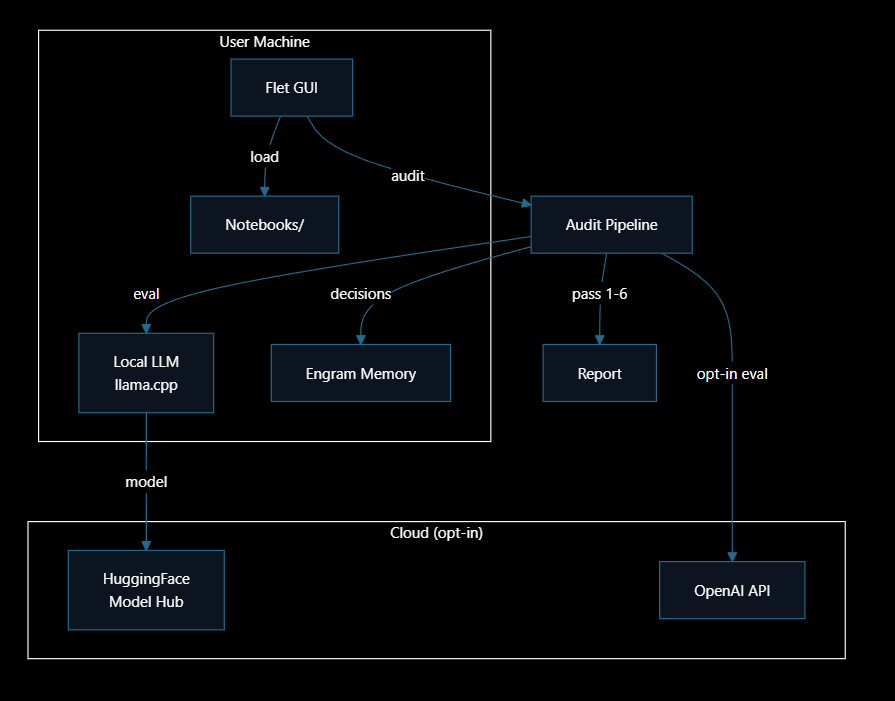
\includegraphics[width=0.85\textwidth]{../../imgs/prd/arquitecturaAltoNivel.png}
\caption{Arquitectura de alto nivel: máquina local + cloud opcional}
\end{figure}

\subsection{Pipeline de Auditoría}

\begin{figure}[h]
\centering
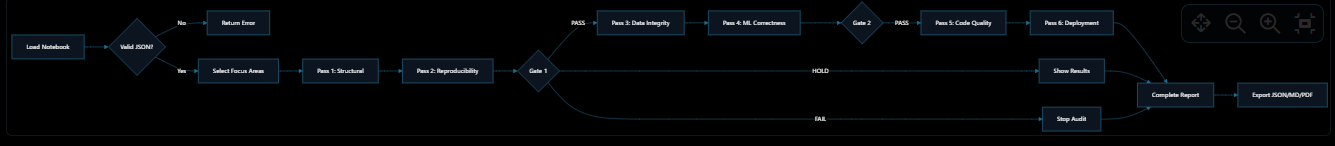
\includegraphics[width=0.92\textwidth]{../../imgs/prd/pipelineAuditoria.png}
\caption{Pipeline de auditoría con gates entre niveles}
\end{figure}

\subsection{Máquina de Estados}

\begin{figure}[h]
\centering
\fbox{%
\begin{minipage}{0.8\textwidth}
\centering
\vspace{6cm}
{\small\textit{[Diagrama Mermaid: Máquina de estados del pipeline de auditoría --- estados IDLE, LOADING, LOADED, AUDITING, PASS1--6, HOLD, COMPLETE, EXPORTING, ERROR]}}
\vspace{6cm}
\end{minipage}%
}
\caption{Máquina de estados del pipeline de auditoría}
\end{figure}

\subsection{LLM Strategy Pattern}

\begin{figure}[h]
\centering
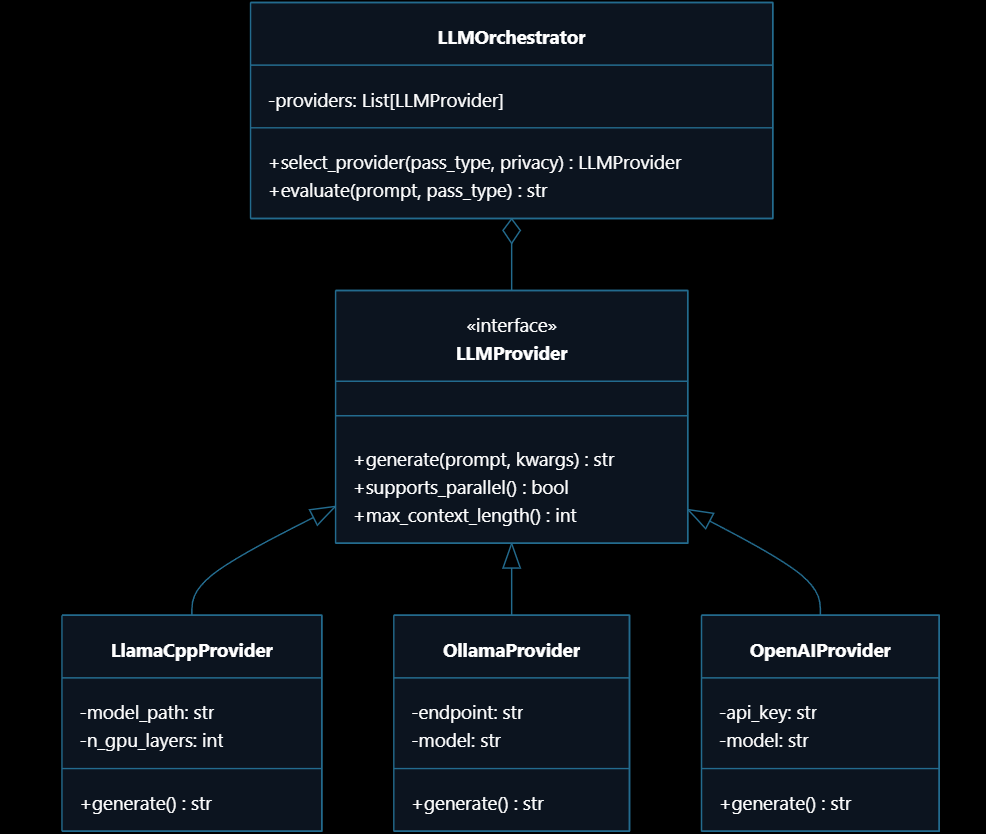
\includegraphics[width=0.78\textwidth]{../../imgs/prd/LLMStrategyPattern.png}
\caption{Diagrama de clases del patrón Strategy para LLM Providers}
\end{figure}

% ==================================================================
\section{Explicación: Ejemplo Completo}
% ==================================================================

Usando \texttt{sample\_audit.ipynb} como caso de prueba, el flujo completo sería:

\subsection{Paso 1: Cargar Notebook}

\begin{verbatim}
$ python main.py
→ Tab: Audit
→ Click: Scan DB
→ Dropdown: sample_audit.ipynb (auto-loaded)
→ Status: "Loaded: sample_audit.ipynb (4 cells)"
\end{verbatim}

\subsection{Paso 2: Seleccionar Focus Areas}

\begin{verbatim}
[o] Structural Overview
[o] Reproducibility Check
[o] Data Integrity Review
[o] ML Correctness Audit
[o] Code Quality Review
[o] Deployment Readiness
\end{verbatim}

\subsection{Paso 3: Ejecutar Auditoría}

\begin{verbatim}
→ Click: Run Audit

Pass 1/6: Structural Overview — PASS
  - 4 cells (1 markdown, 3 code)
  - 1 red flag: cell 3 has null execution_count

Pass 2/6: Reproducibility Check — MODERATE
  - No requirements.txt found
  - Seed set in cell 2: random.seed(42)
  - Risk: MODERATE (missing dep file)

Pass 3/6: Data Integrity Review — PASS
  - No train/test split in notebook → N/A
  - No data loading detected

Pass 4/6: ML Correctness Audit — LOW
  - Simple random sampling, no ML pipeline
  - Score: LOW (no critical issues)

Pass 5/6: Code Quality Review — LOW
  - No repetitive code blocks (>3 threshold)
  - Clear naming, single-purpose cells

Pass 6/6: Deployment Readiness — MODERATE
  - No artifact export detected
  - No environment export file
  - Risk: MODERATE

Audit complete: pass (6 passes)
\end{verbatim}

\subsection{Paso 4: Exportar Reporte}

\begin{verbatim}
→ Click: Export JSON → sample_audit_20260730_120000.json
→ Click: Export PDF → sample_audit_20260730_120000.pdf
\end{verbatim}

\subsection{Resultado Esperado}
\begin{itemize}
  \item 6 tarjetas de resultado visibles en el UI
  \item Cada tarjeta con pass number, pass name, score, finding count
  \item Hallazgos expandibles con detalle por celda
  \item Reportes exportados en formato JSON y PDF
\end{itemize}

% ==================================================================
\section{Anexos}
% ==================================================================

\subsection{Referencias}

\begin{longtable}{llp{0.35\textwidth}}
\toprule
\textbf{Documento} & \textbf{Ubicación} & \textbf{Propósito} \\
\midrule
\endhead
\bottomrule
\endfoot
PRD-AgenticAI-Modular.md        & \texttt{reference/docs/mds/} & PRD completo con 8 módulos y 28 FRs \\
Requirements-AgenticAI.md       & \texttt{reference/docs/mds/} & SRS con 18 FRs, 10 NFRs, 13 TCs \\
DraftGuide.pdf                  & \texttt{reference/docs/pdfs/changes/} & Protocolo Agentic AI (8 building blocks) \\
NotebookBuildAudit.md           & \texttt{reference/docs/mds/} & Construction + Audit frameworks \\
InitialProposalDev.md           & \texttt{reference/docs/mds/} & Propuesta comercial y timeline \\
llmOps.md                       & \texttt{reference/docs/mds/} & LLM-as-a-Judge paradigm \\
ROBINHOOD-Metanym-*-Guide.md    & \texttt{reference/docs/mds/} & Guías de los papers de evaluación \\
agentic-ai-protocol-workflow.pdf & \texttt{reference/docs/latex/requirementsDoc/} & Presentación LaTeX del protocolo \\
forge-auditAgent-requirements.pdf & \texttt{reference/docs/latex/requirementsDoc/} & Presentación LaTeX de requerimientos \\
\bottomrule
\end{longtable}

\subsection{Glosario}

\begin{longtable}{p{0.25\textwidth} p{0.65\textwidth}}
\toprule
\textbf{Término} & \textbf{Definición} \\
\midrule
\endhead
\bottomrule
\endfoot
Agentic AI          & Sistema autónomo que coordina agentes de IA especializados para completar tareas multi-paso \\
LLM-as-a-Judge      & Paradigma donde un LLM evalúa outputs de otro modelo usando criterios cualitativos \\
Construction Framework & Guía de 3 fases para autoría disciplinada de notebooks \\
Audit Framework     & Protocolo de 6 pasadas para revisión sistemática de notebooks \\
Provider Strategy   & Patrón de diseño que permite intercambiar proveedores LLM sin cambiar código cliente \\
HITL                & Human-in-the-Loop: supervisión humana en puntos críticos del flujo \\
CoT                 & Chain-of-Thought: técnica de prompting que encadena razonamiento paso a paso \\
ToT                 & Tree-of-Thoughts: extensión de CoT que explora múltiples caminos de razonamiento \\
SMART               & Specific, Measurable, Achievable, Relevant, Time-bound \\
WBS                 & Work Breakdown Structure: descomposición jerárquica del trabajo \\
RACI                & Responsible, Accountable, Consulted, Informed: matriz de asignación de responsabilidades \\
\bottomrule
\end{longtable}

\subsection{Log de Cambios}

\begin{table}[h]
\centering
\begin{tabular}{lll}
\toprule
\textbf{Versión} & \textbf{Fecha} & \textbf{Cambios} \\
\midrule
v1.0 & 2026-07-30 & Versión inicial del paper de requerimientos \\
\bottomrule
\end{tabular}
\caption{Historial de cambios del documento}
\end{table}

\vfill
\begin{center}
\rule{0.5\textwidth}{0.5pt}\\[4pt]
\small\textit{Documento generado siguiendo el proceso de 9 etapas del protocolo Agentic AI (DraftGuide.pdf) y el ciclo en espiral de Sommerville (Elicitación $\rightarrow$ Especificación $\rightarrow$ Validación).}
\end{center}

\end{document}
